% !TEX TS-program = pdflatex
% !TEX encoding = UTF-8 Unicode
\documentclass[border=0mm]{standalone}
% packages
\usepackage{tikz}
\usetikzlibrary{patterns}
\usepackage{amsmath,amssymb}
\usepackage{bm}
\usepackage{pgfplots}
\pgfplotsset{compat=1.15}
% start document
\begin{document}
% generated by ROOT (CERN)
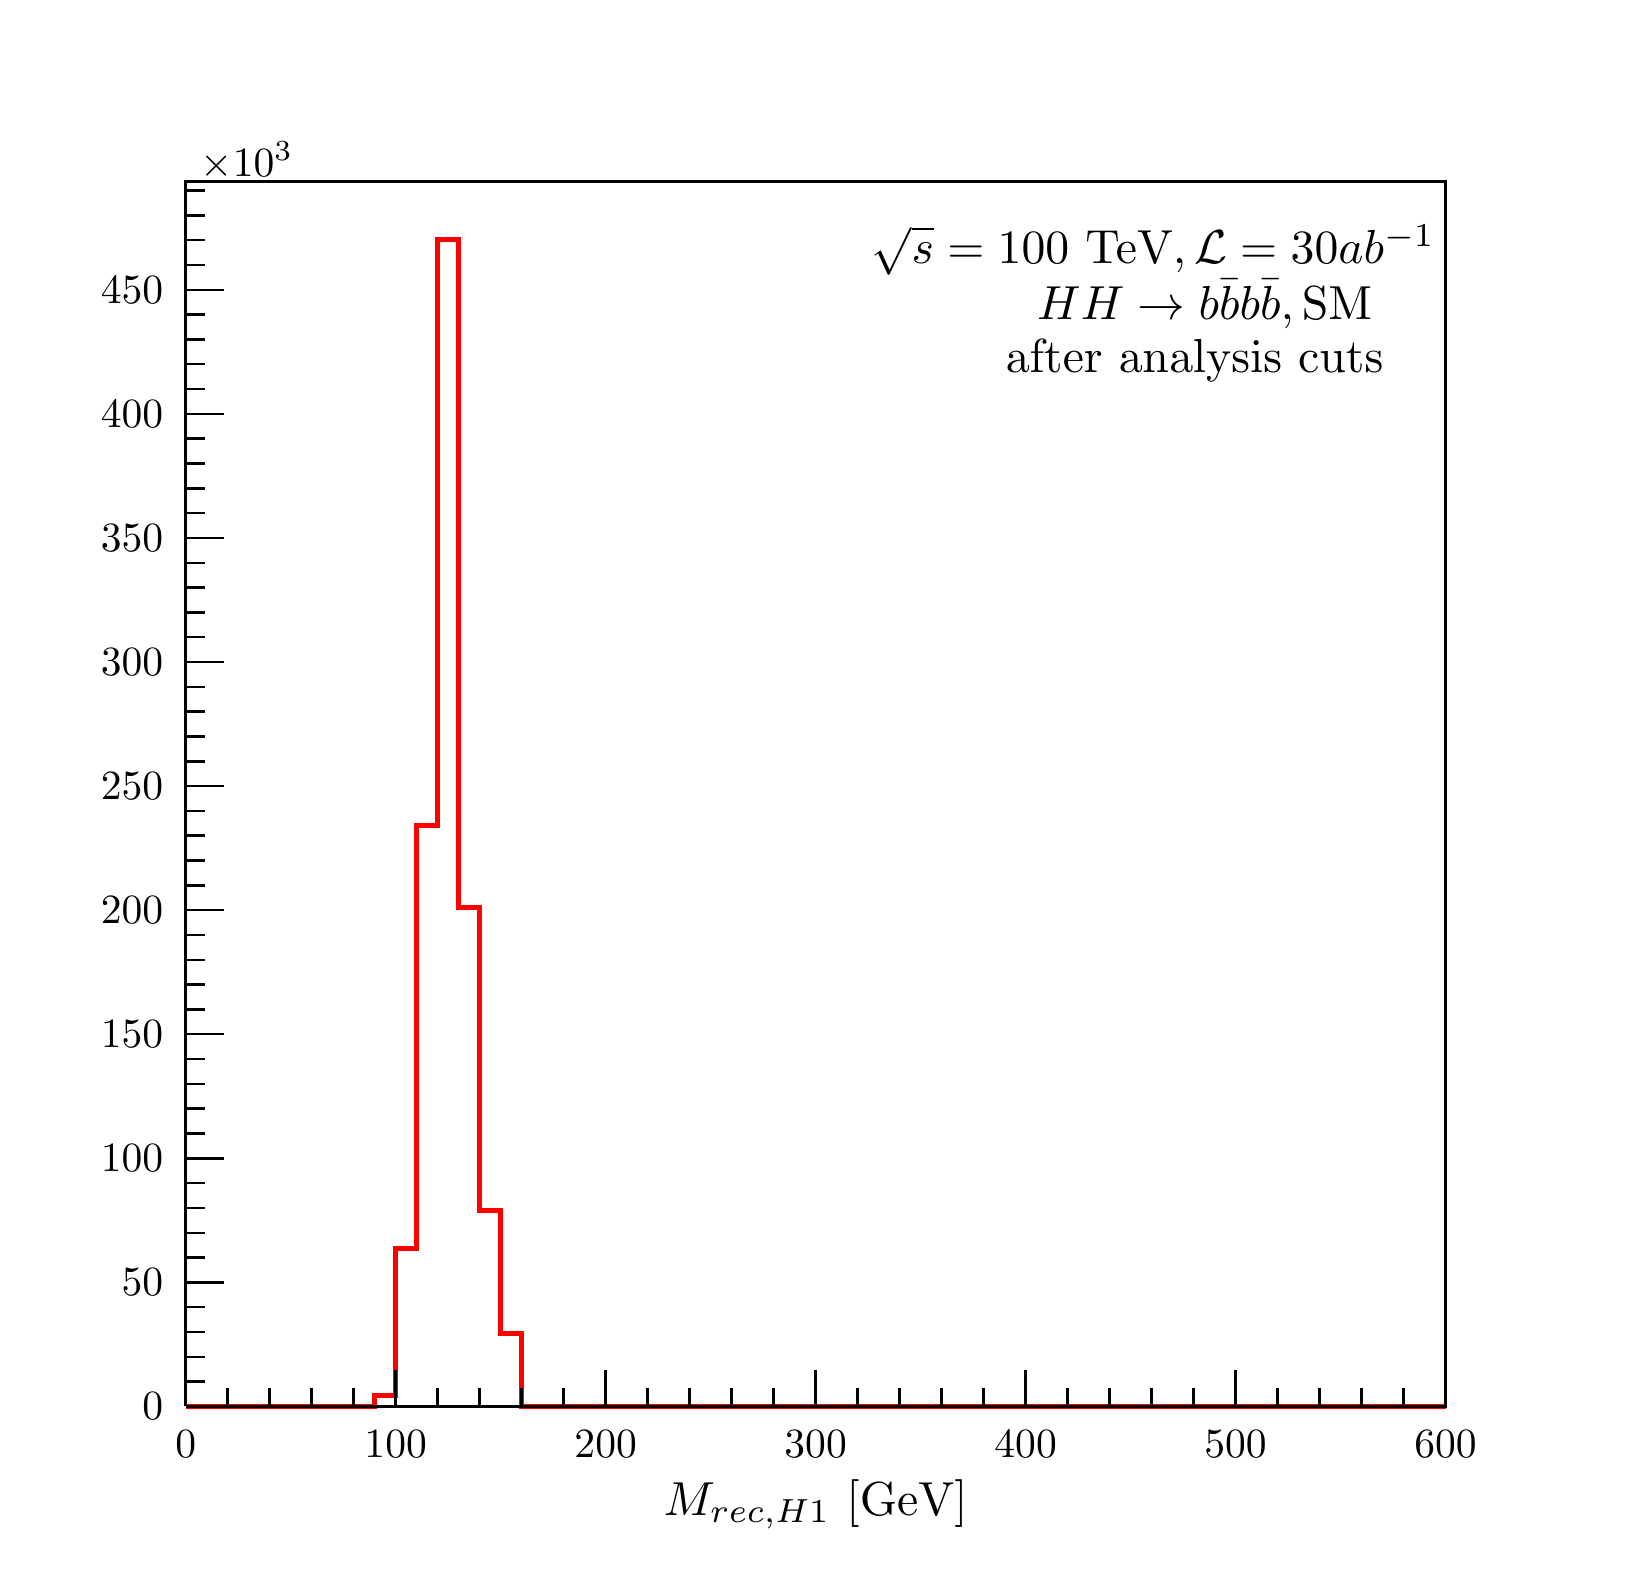
\begin{tikzpicture}
\pgfdeclareplotmark{cross} {
\pgfpathmoveto{\pgfpoint{-0.3\pgfplotmarksize}{\pgfplotmarksize}}
\pgfpathlineto{\pgfpoint{+0.3\pgfplotmarksize}{\pgfplotmarksize}}
\pgfpathlineto{\pgfpoint{+0.3\pgfplotmarksize}{0.3\pgfplotmarksize}}
\pgfpathlineto{\pgfpoint{+1\pgfplotmarksize}{0.3\pgfplotmarksize}}
\pgfpathlineto{\pgfpoint{+1\pgfplotmarksize}{-0.3\pgfplotmarksize}}
\pgfpathlineto{\pgfpoint{+0.3\pgfplotmarksize}{-0.3\pgfplotmarksize}}
\pgfpathlineto{\pgfpoint{+0.3\pgfplotmarksize}{-1.\pgfplotmarksize}}
\pgfpathlineto{\pgfpoint{-0.3\pgfplotmarksize}{-1.\pgfplotmarksize}}
\pgfpathlineto{\pgfpoint{-0.3\pgfplotmarksize}{-0.3\pgfplotmarksize}}
\pgfpathlineto{\pgfpoint{-1.\pgfplotmarksize}{-0.3\pgfplotmarksize}}
\pgfpathlineto{\pgfpoint{-1.\pgfplotmarksize}{0.3\pgfplotmarksize}}
\pgfpathlineto{\pgfpoint{-0.3\pgfplotmarksize}{0.3\pgfplotmarksize}}
\pgfpathclose
\pgfusepathqstroke
}
\pgfdeclareplotmark{cross*} {
\pgfpathmoveto{\pgfpoint{-0.3\pgfplotmarksize}{\pgfplotmarksize}}
\pgfpathlineto{\pgfpoint{+0.3\pgfplotmarksize}{\pgfplotmarksize}}
\pgfpathlineto{\pgfpoint{+0.3\pgfplotmarksize}{0.3\pgfplotmarksize}}
\pgfpathlineto{\pgfpoint{+1\pgfplotmarksize}{0.3\pgfplotmarksize}}
\pgfpathlineto{\pgfpoint{+1\pgfplotmarksize}{-0.3\pgfplotmarksize}}
\pgfpathlineto{\pgfpoint{+0.3\pgfplotmarksize}{-0.3\pgfplotmarksize}}
\pgfpathlineto{\pgfpoint{+0.3\pgfplotmarksize}{-1.\pgfplotmarksize}}
\pgfpathlineto{\pgfpoint{-0.3\pgfplotmarksize}{-1.\pgfplotmarksize}}
\pgfpathlineto{\pgfpoint{-0.3\pgfplotmarksize}{-0.3\pgfplotmarksize}}
\pgfpathlineto{\pgfpoint{-1.\pgfplotmarksize}{-0.3\pgfplotmarksize}}
\pgfpathlineto{\pgfpoint{-1.\pgfplotmarksize}{0.3\pgfplotmarksize}}
\pgfpathlineto{\pgfpoint{-0.3\pgfplotmarksize}{0.3\pgfplotmarksize}}
\pgfpathclose
\pgfusepathqfillstroke
}
\pgfdeclareplotmark{newstar} {
\pgfpathmoveto{\pgfqpoint{0pt}{\pgfplotmarksize}}
\pgfpathlineto{\pgfqpointpolar{44}{0.5\pgfplotmarksize}}
\pgfpathlineto{\pgfqpointpolar{18}{\pgfplotmarksize}}
\pgfpathlineto{\pgfqpointpolar{-20}{0.5\pgfplotmarksize}}
\pgfpathlineto{\pgfqpointpolar{-54}{\pgfplotmarksize}}
\pgfpathlineto{\pgfqpointpolar{-90}{0.5\pgfplotmarksize}}
\pgfpathlineto{\pgfqpointpolar{234}{\pgfplotmarksize}}
\pgfpathlineto{\pgfqpointpolar{198}{0.5\pgfplotmarksize}}
\pgfpathlineto{\pgfqpointpolar{162}{\pgfplotmarksize}}
\pgfpathlineto{\pgfqpointpolar{134}{0.5\pgfplotmarksize}}
\pgfpathclose
\pgfusepathqstroke
}
\pgfdeclareplotmark{newstar*} {
\pgfpathmoveto{\pgfqpoint{0pt}{\pgfplotmarksize}}
\pgfpathlineto{\pgfqpointpolar{44}{0.5\pgfplotmarksize}}
\pgfpathlineto{\pgfqpointpolar{18}{\pgfplotmarksize}}
\pgfpathlineto{\pgfqpointpolar{-20}{0.5\pgfplotmarksize}}
\pgfpathlineto{\pgfqpointpolar{-54}{\pgfplotmarksize}}
\pgfpathlineto{\pgfqpointpolar{-90}{0.5\pgfplotmarksize}}
\pgfpathlineto{\pgfqpointpolar{234}{\pgfplotmarksize}}
\pgfpathlineto{\pgfqpointpolar{198}{0.5\pgfplotmarksize}}
\pgfpathlineto{\pgfqpointpolar{162}{\pgfplotmarksize}}
\pgfpathlineto{\pgfqpointpolar{134}{0.5\pgfplotmarksize}}
\pgfpathclose
\pgfusepathqfillstroke
}
\definecolor{c}{rgb}{1,1,1};
\draw [color=c, fill=c] (0,0) rectangle (20,19.4486);
\draw [color=c, fill=c] (0,0) rectangle (20,19.4486);
\draw [color=c, fill=c] (2,1.94486) rectangle (18,17.5038);
\definecolor{c}{rgb}{0,0,0};
\draw [c,line width=0.9] (2,1.94486) -- (2,17.5038) -- (18,17.5038) -- (18,1.94486) -- (2,1.94486);
\definecolor{c}{rgb}{1,1,1};
\draw [color=c, fill=c] (2,1.94486) rectangle (18,17.5038);
\definecolor{c}{rgb}{0,0,0};
\draw [c,line width=0.9] (2,1.94486) -- (2,17.5038) -- (18,17.5038) -- (18,1.94486) -- (2,1.94486);
\definecolor{c}{rgb}{1,0,0};
\draw [c,line width=1.8] (2,1.94486) -- (2.26667,1.94486) -- (2.26667,1.94486) -- (2.53333,1.94486) -- (2.53333,1.94486) -- (2.8,1.94486) -- (2.8,1.94486) -- (3.06667,1.94486) -- (3.06667,1.94486) -- (3.33333,1.94486) -- (3.33333,1.94486) --
 (3.6,1.94486) -- (3.6,1.94486) -- (3.86667,1.94486) -- (3.86667,1.94486) -- (4.13333,1.94486) -- (4.13333,1.94486) -- (4.4,1.94486) -- (4.4,2.07878) -- (4.66667,2.07878) -- (4.66667,3.95594) -- (4.93333,3.95594) -- (4.93333,9.32428) -- (5.2,9.32428)
 -- (5.2,16.7629) -- (5.46667,16.7629) -- (5.46667,8.27708) -- (5.73333,8.27708) -- (5.73333,4.43321) -- (6,4.43321) -- (6,2.87527) -- (6.26667,2.87527) -- (6.26667,1.94486) -- (6.53333,1.94486) -- (6.53333,1.94486) -- (6.8,1.94486) -- (6.8,1.94486)
 -- (7.06667,1.94486) -- (7.06667,1.94486) -- (7.33333,1.94486) -- (7.33333,1.94486) -- (7.6,1.94486) -- (7.6,1.94486) -- (7.86667,1.94486) -- (7.86667,1.94486) -- (8.13333,1.94486) -- (8.13333,1.94486) -- (8.4,1.94486) -- (8.4,1.94486) --
 (8.66667,1.94486) -- (8.66667,1.94486) -- (8.93333,1.94486) -- (8.93333,1.94486) -- (9.2,1.94486) -- (9.2,1.94486) -- (9.46667,1.94486) -- (9.46667,1.94486) -- (9.73333,1.94486) -- (9.73333,1.94486) -- (10,1.94486) -- (10,1.94486) --
 (10.2667,1.94486) -- (10.2667,1.94486) -- (10.5333,1.94486) -- (10.5333,1.94486) -- (10.8,1.94486) -- (10.8,1.94486) -- (11.0667,1.94486) -- (11.0667,1.94486) -- (11.3333,1.94486) -- (11.3333,1.94486) -- (11.6,1.94486) -- (11.6,1.94486) --
 (11.8667,1.94486) -- (11.8667,1.94486) -- (12.1333,1.94486) -- (12.1333,1.94486) -- (12.4,1.94486) -- (12.4,1.94486) -- (12.6667,1.94486) -- (12.6667,1.94486) -- (12.9333,1.94486) -- (12.9333,1.94486) -- (13.2,1.94486) -- (13.2,1.94486) --
 (13.4667,1.94486) -- (13.4667,1.94486) -- (13.7333,1.94486) -- (13.7333,1.94486) -- (14,1.94486) -- (14,1.94486) -- (14.2667,1.94486) -- (14.2667,1.94486) -- (14.5333,1.94486) -- (14.5333,1.94486) -- (14.8,1.94486) -- (14.8,1.94486) --
 (15.0667,1.94486) -- (15.0667,1.94486) -- (15.3333,1.94486) -- (15.3333,1.94486) -- (15.6,1.94486) -- (15.6,1.94486) -- (15.8667,1.94486) -- (15.8667,1.94486) -- (16.1333,1.94486) -- (16.1333,1.94486) -- (16.4,1.94486) -- (16.4,1.94486) --
 (16.6667,1.94486) -- (16.6667,1.94486) -- (16.9333,1.94486) -- (16.9333,1.94486) -- (17.2,1.94486) -- (17.2,1.94486) -- (17.4667,1.94486) -- (17.4667,1.94486) -- (17.7333,1.94486) -- (17.7333,1.94486) -- (18,1.94486);
\definecolor{c}{rgb}{0,0,0};
\draw [c,line width=0.9] (2,1.94486) -- (18,1.94486);
\draw [c,line width=0.9] (2,2.41163) -- (2,1.94486);
\draw [c,line width=0.9] (2.53333,2.17825) -- (2.53333,1.94486);
\draw [c,line width=0.9] (3.06667,2.17825) -- (3.06667,1.94486);
\draw [c,line width=0.9] (3.6,2.17825) -- (3.6,1.94486);
\draw [c,line width=0.9] (4.13333,2.17825) -- (4.13333,1.94486);
\draw [c,line width=0.9] (4.66667,2.41163) -- (4.66667,1.94486);
\draw [c,line width=0.9] (5.2,2.17825) -- (5.2,1.94486);
\draw [c,line width=0.9] (5.73333,2.17825) -- (5.73333,1.94486);
\draw [c,line width=0.9] (6.26667,2.17825) -- (6.26667,1.94486);
\draw [c,line width=0.9] (6.8,2.17825) -- (6.8,1.94486);
\draw [c,line width=0.9] (7.33333,2.41163) -- (7.33333,1.94486);
\draw [c,line width=0.9] (7.86667,2.17825) -- (7.86667,1.94486);
\draw [c,line width=0.9] (8.4,2.17825) -- (8.4,1.94486);
\draw [c,line width=0.9] (8.93333,2.17825) -- (8.93333,1.94486);
\draw [c,line width=0.9] (9.46667,2.17825) -- (9.46667,1.94486);
\draw [c,line width=0.9] (10,2.41163) -- (10,1.94486);
\draw [c,line width=0.9] (10.5333,2.17825) -- (10.5333,1.94486);
\draw [c,line width=0.9] (11.0667,2.17825) -- (11.0667,1.94486);
\draw [c,line width=0.9] (11.6,2.17825) -- (11.6,1.94486);
\draw [c,line width=0.9] (12.1333,2.17825) -- (12.1333,1.94486);
\draw [c,line width=0.9] (12.6667,2.41163) -- (12.6667,1.94486);
\draw [c,line width=0.9] (13.2,2.17825) -- (13.2,1.94486);
\draw [c,line width=0.9] (13.7333,2.17825) -- (13.7333,1.94486);
\draw [c,line width=0.9] (14.2667,2.17825) -- (14.2667,1.94486);
\draw [c,line width=0.9] (14.8,2.17825) -- (14.8,1.94486);
\draw [c,line width=0.9] (15.3333,2.41163) -- (15.3333,1.94486);
\draw [c,line width=0.9] (15.8667,2.17825) -- (15.8667,1.94486);
\draw [c,line width=0.9] (16.4,2.17825) -- (16.4,1.94486);
\draw [c,line width=0.9] (16.9333,2.17825) -- (16.9333,1.94486);
\draw [c,line width=0.9] (17.4667,2.17825) -- (17.4667,1.94486);
\draw [c,line width=0.9] (18,2.41163) -- (18,1.94486);
\draw [anchor=base] (2,1.30306) node[scale=1.50291, color=c, rotate=0]{0};
\draw [anchor=base] (4.66667,1.30306) node[scale=1.50291, color=c, rotate=0]{100};
\draw [anchor=base] (7.33333,1.30306) node[scale=1.50291, color=c, rotate=0]{200};
\draw [anchor=base] (10,1.30306) node[scale=1.50291, color=c, rotate=0]{300};
\draw [anchor=base] (12.6667,1.30306) node[scale=1.50291, color=c, rotate=0]{400};
\draw [anchor=base] (15.3333,1.30306) node[scale=1.50291, color=c, rotate=0]{500};
\draw [anchor=base] (18,1.30306) node[scale=1.50291, color=c, rotate=0]{600};
\draw (10,0.700151) node[scale=1.72557, color=c, rotate=0]{$M_{rec, H1} ~[\text{GeV}]$};
\draw [c,line width=0.9] (2,1.94486) -- (2,17.5038);
\draw [c,line width=0.9] (2.48,1.94486) -- (2,1.94486);
\draw [c,line width=0.9] (2.24,2.26001) -- (2,2.26001);
\draw [c,line width=0.9] (2.24,2.57516) -- (2,2.57516);
\draw [c,line width=0.9] (2.24,2.89031) -- (2,2.89031);
\draw [c,line width=0.9] (2.24,3.20546) -- (2,3.20546);
\draw [c,line width=0.9] (2.48,3.52061) -- (2,3.52061);
\draw [c,line width=0.9] (2.24,3.83576) -- (2,3.83576);
\draw [c,line width=0.9] (2.24,4.15091) -- (2,4.15091);
\draw [c,line width=0.9] (2.24,4.46606) -- (2,4.46606);
\draw [c,line width=0.9] (2.24,4.78121) -- (2,4.78121);
\draw [c,line width=0.9] (2.48,5.09636) -- (2,5.09636);
\draw [c,line width=0.9] (2.24,5.41151) -- (2,5.41151);
\draw [c,line width=0.9] (2.24,5.72665) -- (2,5.72665);
\draw [c,line width=0.9] (2.24,6.0418) -- (2,6.0418);
\draw [c,line width=0.9] (2.24,6.35695) -- (2,6.35695);
\draw [c,line width=0.9] (2.48,6.6721) -- (2,6.6721);
\draw [c,line width=0.9] (2.24,6.98725) -- (2,6.98725);
\draw [c,line width=0.9] (2.24,7.3024) -- (2,7.3024);
\draw [c,line width=0.9] (2.24,7.61755) -- (2,7.61755);
\draw [c,line width=0.9] (2.24,7.9327) -- (2,7.9327);
\draw [c,line width=0.9] (2.48,8.24785) -- (2,8.24785);
\draw [c,line width=0.9] (2.24,8.563) -- (2,8.563);
\draw [c,line width=0.9] (2.24,8.87815) -- (2,8.87815);
\draw [c,line width=0.9] (2.24,9.1933) -- (2,9.1933);
\draw [c,line width=0.9] (2.24,9.50845) -- (2,9.50845);
\draw [c,line width=0.9] (2.48,9.8236) -- (2,9.8236);
\draw [c,line width=0.9] (2.24,10.1387) -- (2,10.1387);
\draw [c,line width=0.9] (2.24,10.4539) -- (2,10.4539);
\draw [c,line width=0.9] (2.24,10.769) -- (2,10.769);
\draw [c,line width=0.9] (2.24,11.0842) -- (2,11.0842);
\draw [c,line width=0.9] (2.48,11.3993) -- (2,11.3993);
\draw [c,line width=0.9] (2.24,11.7145) -- (2,11.7145);
\draw [c,line width=0.9] (2.24,12.0296) -- (2,12.0296);
\draw [c,line width=0.9] (2.24,12.3448) -- (2,12.3448);
\draw [c,line width=0.9] (2.24,12.6599) -- (2,12.6599);
\draw [c,line width=0.9] (2.48,12.9751) -- (2,12.9751);
\draw [c,line width=0.9] (2.24,13.2902) -- (2,13.2902);
\draw [c,line width=0.9] (2.24,13.6054) -- (2,13.6054);
\draw [c,line width=0.9] (2.24,13.9205) -- (2,13.9205);
\draw [c,line width=0.9] (2.24,14.2357) -- (2,14.2357);
\draw [c,line width=0.9] (2.48,14.5508) -- (2,14.5508);
\draw [c,line width=0.9] (2.24,14.866) -- (2,14.866);
\draw [c,line width=0.9] (2.24,15.1811) -- (2,15.1811);
\draw [c,line width=0.9] (2.24,15.4963) -- (2,15.4963);
\draw [c,line width=0.9] (2.24,15.8114) -- (2,15.8114);
\draw [c,line width=0.9] (2.48,16.1266) -- (2,16.1266);
\draw [c,line width=0.9] (2.48,16.1266) -- (2,16.1266);
\draw [c,line width=0.9] (2.24,16.4417) -- (2,16.4417);
\draw [c,line width=0.9] (2.24,16.7569) -- (2,16.7569);
\draw [c,line width=0.9] (2.24,17.072) -- (2,17.072);
\draw [c,line width=0.9] (2.24,17.3872) -- (2,17.3872);
\draw [anchor= east] (1.9,1.94486) node[scale=1.50291, color=c, rotate=0]{0};
\draw [anchor= east] (1.9,3.52061) node[scale=1.50291, color=c, rotate=0]{50};
\draw [anchor= east] (1.9,5.09636) node[scale=1.50291, color=c, rotate=0]{100};
\draw [anchor= east] (1.9,6.6721) node[scale=1.50291, color=c, rotate=0]{150};
\draw [anchor= east] (1.9,8.24785) node[scale=1.50291, color=c, rotate=0]{200};
\draw [anchor= east] (1.9,9.8236) node[scale=1.50291, color=c, rotate=0]{250};
\draw [anchor= east] (1.9,11.3993) node[scale=1.50291, color=c, rotate=0]{300};
\draw [anchor= east] (1.9,12.9751) node[scale=1.50291, color=c, rotate=0]{350};
\draw [anchor= east] (1.9,14.5508) node[scale=1.50291, color=c, rotate=0]{400};
\draw [anchor= east] (1.9,16.1266) node[scale=1.50291, color=c, rotate=0]{450};
\draw [anchor=base west] (2,17.5718) node[scale=1.50291, color=c, rotate=0]{$\times10^{3}$};
\draw [anchor= west] (10.5,16.6286) node[scale=1.72557, color=c, rotate=0]{$\sqrt{s} = 100 ~\text{TeV}, \mathcal{L} = 30 ab^{-1}$};
\draw [anchor= west] (12.6,15.9479) node[scale=1.72557, color=c, rotate=0]{$HH \rightarrow b\bar{b}b\bar{b},\text{SM}$};
\draw [anchor=base west] (12.2,15.0824) node[scale=1.72557, color=c, rotate=0]{after analysis cuts};
\end{tikzpicture}
% end document
\end{document}
